\Gls{tic} is a tool fully devoted to the \gls{tc} \gls{rnaseq} data offering features to inspect the data, to normalize them, to capture the differential expression of genes at the static time point and overall time points, supporting different experimental designs.
It is also possible to compare the results coming from different analysis and to investigate the most influenced biological functions (i.e. Gene Ontology terms and Pathways \cite{GeneOntologyConsortium2004, GeneOntologyConsortium2015} ).

Overall, \gls{tic} offers the possibility to analyze data using different R/Bioconductor \cite{Gentleman2004} packages, to compare the results in order to choose the best combination of tools for the user specific problem. Therefore, the software implements a vast amount of exploratory and diagnostic interactive plots to explore data not just at pre-processing step but also during the post-processing phase. 

%\gls{tic} automatically implements a set of Reproducible Research functionalities to trace all the analysis steps selected by the user, generating a final report with both executed analysis code chunks and their produced results. Furthermore, \gls{tic} has been provided also of a caching system providing, for each analysis step, a caching database file within all the input and output processed data, useful, not only to speed up computations, but also to share data and results through the Internet.

\begin{figure}[h]
\centering
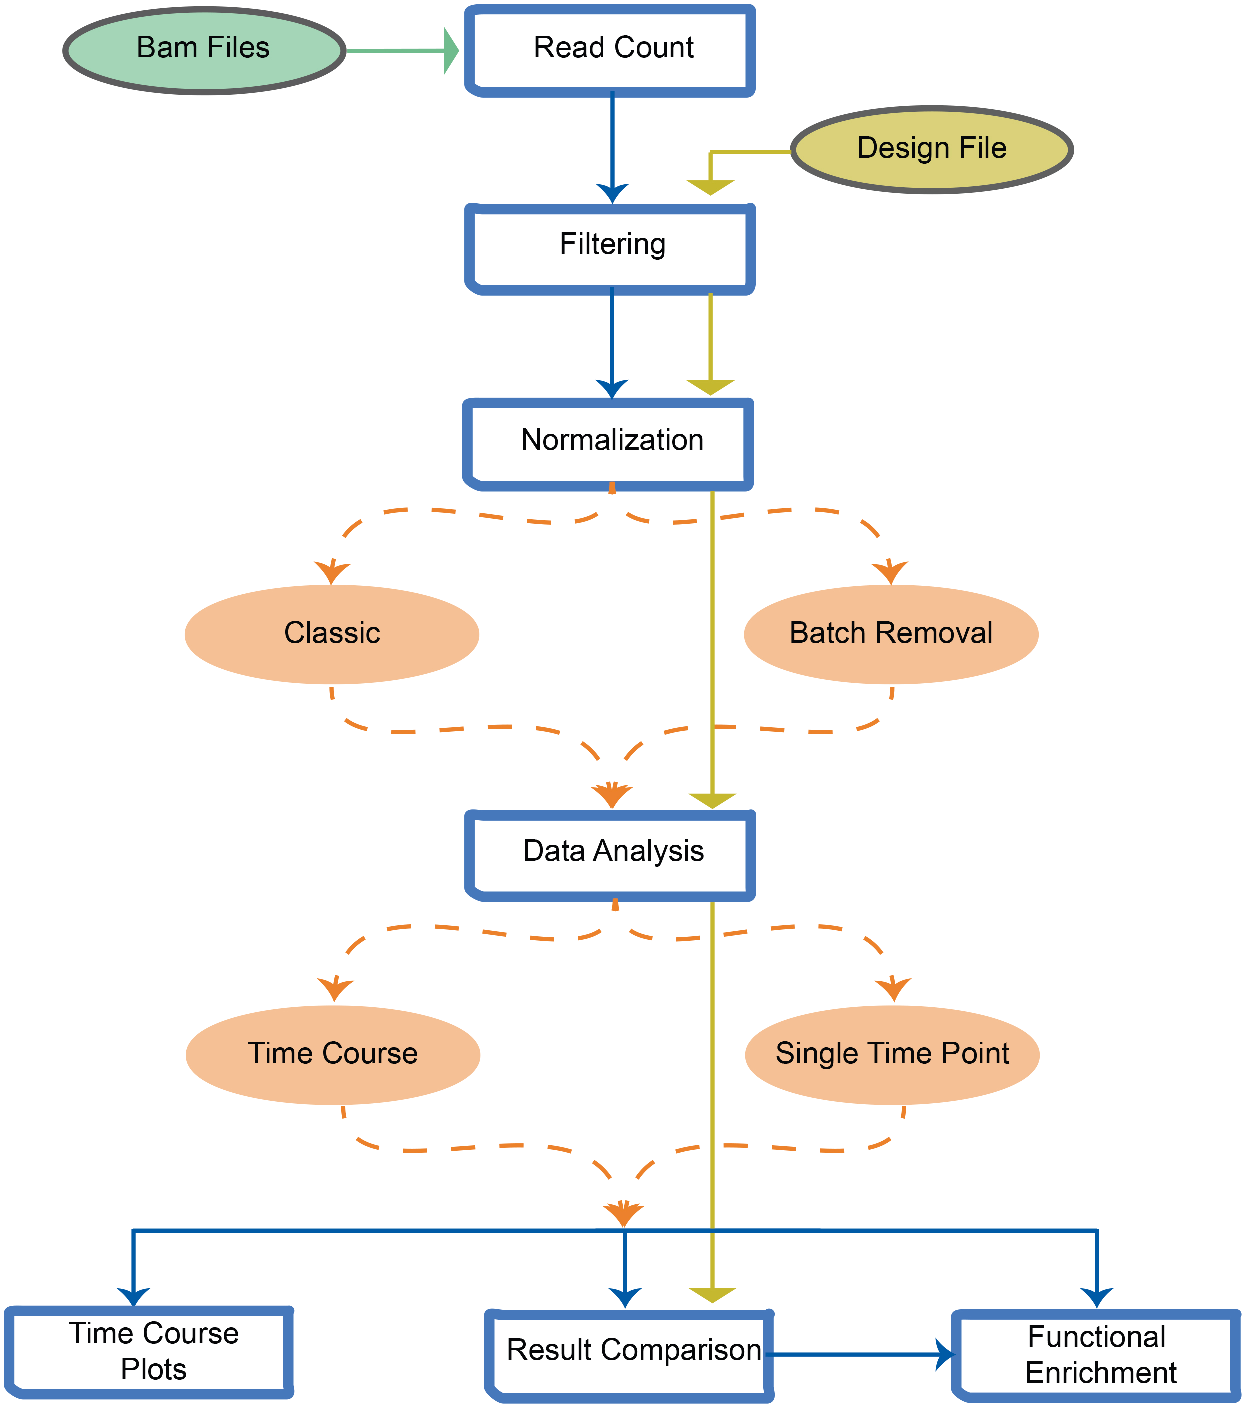
\includegraphics[width=8cm, keepaspectratio]{img/ticorser/main_flow.pdf}
\caption[ticorser mainflow]{Main flow of ticorser R package.
The package takes as input a list of bam files for producing a count matrix of the features (on the rows) and the samples (on the columns).
Afterwards, with aid of a design file, \gls{tic} allows the filtering of low expressed genomic features and their normalization with classic methodologies and with spefici ones for batch removal.
Once the data are comparable it is possible to perform a differential expression at time-course level and/or at specific time point.
The results can be investigated for plotting, comparison or for functional enrichment.}
\label{fig:ticorserflow}
\end{figure}

Starting the analysis of \gls{tc} \gls{rnaseq} data from \gls{bam} files, \gls{tic} enables \gls{rna} expression quantification through \lstinline!featureCounts! method \cite{Liao2014}, producing a count matrix of features per samples, which enables the \glspl{deg} detection with hypothesis statistical methods.

As figure \ref{fig:ticorserflow} shows, this is a \textit{design file based} tool, where a file, that describes all the samples by several variables, chaperons the count matrix through all the analysis, simplifying, in such a way, the user interaction with all the available instruments.
 
Particular attention is given to the normalization phase, providing the possibility not only to use several traditional normalization methods but also the methodologies for batch effect removal.

In oder to inspect different approaches to analyze \gls{tc} data, \gls{tic} offers three different methodologies for analyzing \gls{tc} \gls{rnaseq} data, and four different methods to analyze different biological conditions at single time point level.

